\documentclass{article}

\usepackage[T1]{fontenc}
\usepackage[spanish,es-nodecimaldot]{babel}
\usepackage{graphicx}
\usepackage{fancyhdr}
\usepackage[top=2.5cm,bottom=2cm,left=2.5cm,right=2.5cm,headheight=1.2cm,headsep=0.3cm]{geometry}
\usepackage{float}
\usepackage{array}
\usepackage{tabularx}
\usepackage[table]{xcolor}
\usepackage{listings}
\usepackage{caption}
\usepackage[hidelinks]{hyperref}

\definecolor{tableblack}{RGB}{0,0,0}
\definecolor{tablewhite}{RGB}{255,255,255}
\newcolumntype{Y}{>{\raggedright\arraybackslash}X}

\pagestyle{fancy}
\fancyhf{}
\fancyhead[L]{
\includegraphics[width=1cm]{espol.png}}
\fancyhead[R]{
\includegraphics[width=1cm]{fiec.png}}
\fancyfoot[C]{\thepage}
\renewcommand{\headrulewidth}{0pt}
\renewcommand{\footrulewidth}{0pt}

\hypersetup{
  pdftitle={Tarea 6 - Gestión de Energía en el ESP32},
  pdfauthor={Jandony Guzman Garofalo},
  pdfsubject={Sistemas Embebidos},
  colorlinks=false
}

\lstset{
  language=C++,
  basicstyle=\ttfamily\footnotesize,
  frame=single,
  rulecolor=\color{black},
  backgroundcolor=\color{white},
  keywordstyle=\bfseries,
  commentstyle=\itshape,
  stringstyle=\normalfont\ttfamily,
  numbers=none,
  breaklines=true,
  showstringspaces=false,
  columns=fullflexible,
  keepspaces=true,
  aboveskip=0.8em,
  belowskip=0.8em
}

\newcommand{\tableheader}[1]{\color{tablewhite}\textbf{#1}}

\begin{document}

\noindent\textbf{Nombre del estudiante:} Jandony Guzman Garofalo

\vspace{0.5em}
\noindent\textbf{Paralelo:} 1

\vspace{1em}
\begin{center}
  \textbf{REPORTE \#6}\\[0.5em]
  \textbf{GESTIÓN DE ENERGÍA EN EL ESP32}
\end{center}

\vspace{1em}

\section{Descripción del ejercicio}

En este trabajo implementé un sistema que ejecuta una tarea durante cinco segundos y luego entra en modo \textit{deep sleep}. El ESP32 puede despertar de dos formas: automáticamente mediante el temporizador RTC o al presionar un pulsador conectado al GPIO33. El estado del sistema se muestra con un LED RGB y también se escribe en el monitor serial.

Escogí \textit{deep sleep} porque en este modo la CPU y la mayoría de los periféricos digitales dejan de funcionar. Solo se mantienen los elementos del dominio RTC que se necesitan para conservar los contadores y detectar las fuentes de despertar.

\subsection{Objetivos de la implementación}

\begin{itemize}
  \item Ejecutar una tarea activa durante un tiempo definido.
  \item Configurar el despertar por temporizador con \texttt{esp\_sleep\_enable\_timer\_wakeup()}.
  \item Configurar el despertar externo con \texttt{esp\_sleep\_enable\_ext0\_wakeup()}.
  \item Indicar los estados mediante un LED RGB y mensajes seriales.
  \item Organizar el código en funciones y archivos separados.
\end{itemize}

\section{Circuito en Wokwi}

El circuito utiliza un ESP32 DevKit v1, un LED RGB de cátodo común, tres resistencias de 220~$\Omega$, un pulsador y una resistencia de 10~k$\Omega$ para mantener el GPIO33 en nivel alto mientras el botón no está presionado.

\begin{figure}[H]
  \centering
  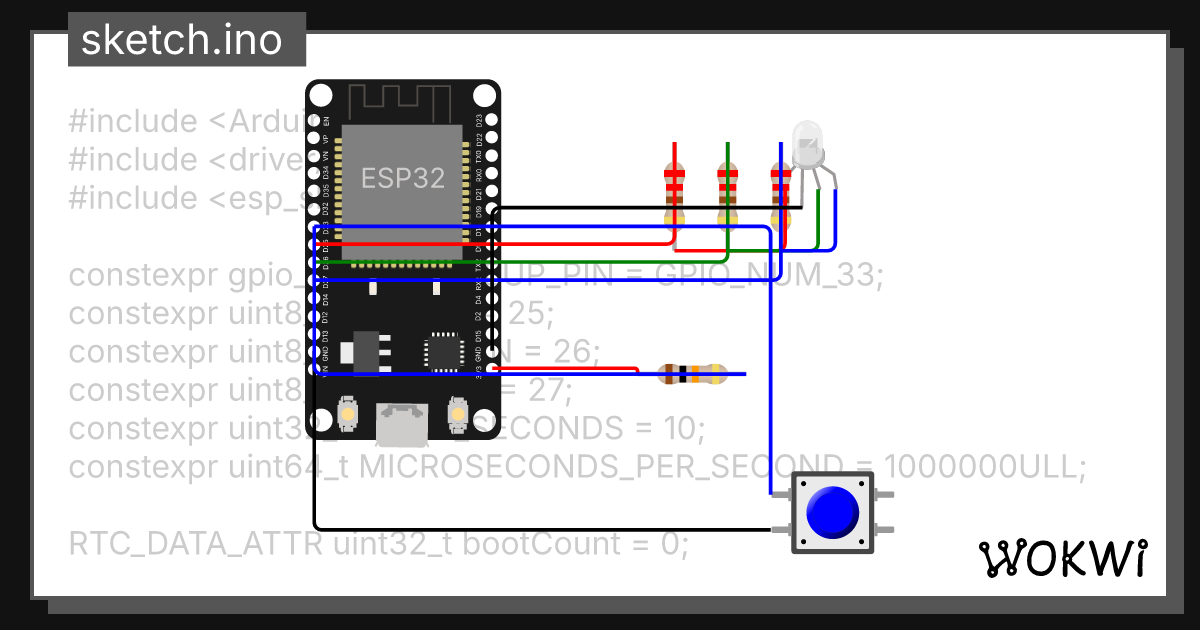
\includegraphics[width=0.95\linewidth]{img/circuito-wokwi.png}
  \caption{Circuito implementado y publicado en Wokwi.}
  \label{fig:circuito_wokwi}
\end{figure}

\begin{table}[H]
\centering
\renewcommand{\arraystretch}{1.25}
\begin{tabularx}{\linewidth}{|p{3.2cm}|p{5.3cm}|Y|}
\hline
\rowcolor{tableblack}\tableheader{Elemento} & \tableheader{Conexión} & \tableheader{Uso} \\
\hline
Canal rojo & GPIO25, resistencia de 220~$\Omega$ y pin R & Preparación para dormir \\
\hline
Canal verde & GPIO26, resistencia de 220~$\Omega$ y pin G & Tarea activa \\
\hline
Canal azul & GPIO27, resistencia de 220~$\Omega$ y pin B & Arranque o despertar \\
\hline
Pulsador & GPIO33 y GND & Despertar externo EXT0 \\
\hline
Resistencia pull-up & 3.3~V, 10~k$\Omega$ y GPIO33 & Mantener el pin en HIGH \\
\hline
\end{tabularx}
\caption{Conexiones principales del circuito.}
\end{table}

El circuito se puede abrir desde el siguiente vínculo: \href{https://wokwi.com/projects/471748304593999873}{\textbf{proyecto en Wokwi}}. Durante el reposo se puede hacer clic en el pulsador azul o mantener presionada la tecla \texttt{B}.

\section{Funcionamiento del sistema}

La secuencia se repite después de cada despertar:

\begin{enumerate}
  \item El ESP32 inicia, lee la causa del arranque y enciende el LED azul.
  \item Ejecuta la tarea activa durante cinco segundos. El LED verde parpadea una vez por segundo.
  \item Enciende los canales rojo y verde al mismo tiempo para formar amarillo. En ese momento configura TIMER y EXT0.
  \item Apaga el LED y entra en \textit{deep sleep}.
  \item Despierta al cumplirse diez segundos o cuando GPIO33 pasa a nivel bajo.
\end{enumerate}

\begin{table}[H]
\centering
\renewcommand{\arraystretch}{1.25}
\begin{tabularx}{\linewidth}{|p{3.4cm}|p{3.4cm}|Y|}
\hline
\rowcolor{tableblack}\tableheader{Estado} & \tableheader{LED} & \tableheader{Mensaje principal} \\
\hline
Despierto & Azul & \texttt{ESTADO=DESPIERTO} \\
\hline
Tarea activa & Verde intermitente & \texttt{ESTADO=ACTIVO} \\
\hline
Preparando reposo & Amarillo & \texttt{ESTADO=PREPARANDO\_SLEEP} \\
\hline
Deep sleep & Apagado & \texttt{ESTADO=SLEEP} \\
\hline
\end{tabularx}
\caption{Estados indicados por el LED y el monitor serial.}
\end{table}

\subsection{Memoria RTC}

El despertar desde \textit{deep sleep} reinicia la ejecución desde \texttt{setup()}. Para comprobar que existió un ciclo anterior, declaré tres contadores con \texttt{RTC\_DATA\_ATTR}. Estos datos se mantienen mientras el dominio RTC siga alimentado.

\begin{lstlisting}
RTC_DATA_ATTR uint32_t bootCount = 0;
RTC_DATA_ATTR uint32_t timerWakeCount = 0;
RTC_DATA_ATTR uint32_t externalWakeCount = 0;
\end{lstlisting}

\section{Desarrollo del código}

El proyecto principal se desarrolló en PlatformIO con el framework Arduino. Separé el manejo del LED y la configuración de energía para que el archivo principal solo contenga la secuencia del ejercicio.

\begin{table}[H]
\centering
\renewcommand{\arraystretch}{1.25}
\begin{tabularx}{\linewidth}{|p{5cm}|Y|}
\hline
\rowcolor{tableblack}\tableheader{Archivo} & \tableheader{Contenido} \\
\hline
\texttt{src/main.cpp} & Flujo principal, tarea activa y contadores RTC. \\
\hline
\texttt{src/power\_manager.cpp} & Fuentes de despertar y entrada a deep sleep. \\
\hline
\texttt{src/status\_led.cpp} & Control de los canales del LED RGB. \\
\hline
\texttt{diagram.json} & Componentes y conexiones del circuito Wokwi. \\
\hline
\texttt{wokwi.toml} & Rutas del firmware generado por PlatformIO. \\
\hline
\texttt{tests/} & Escenarios TIMER, EXT0 y validación del proyecto. \\
\hline
\end{tabularx}
\caption{Organización del proyecto.}
\end{table}

La configuración de las fuentes de despertar se realiza antes de apagar el LED y entrar en reposo:

\begin{lstlisting}
esp_sleep_enable_timer_wakeup(
    SLEEP_SECONDS * MICROSECONDS_PER_SECOND);

esp_sleep_enable_ext0_wakeup(
    GPIO_NUM_33, LOW);

rtc_gpio_pullup_en(GPIO_NUM_33);
rtc_gpio_pulldown_dis(GPIO_NUM_33);

esp_deep_sleep_start();
\end{lstlisting}

Antes de ejecutar \texttt{esp\_deep\_sleep\_start()}, el programa espera que el botón esté liberado. Esto evita que el ESP32 se duerma con la condición EXT0 ya activa y se despierte de inmediato.

\section{Pruebas realizadas}

Primero compilé el proyecto completo con PlatformIO. También compilé por separado el archivo usado en la versión web de Wokwi para comprobar que ambas variantes sean válidas. Finalmente, revisé el archivo \texttt{diagram.json} con el linter de Wokwi y ejecuté un script que compara los pines del circuito con los pines usados en el código.

\begin{table}[H]
\centering
\renewcommand{\arraystretch}{1.25}
\begin{tabularx}{\linewidth}{|Y|p{3.2cm}|p{5.3cm}|}
\hline
\rowcolor{tableblack}\tableheader{Prueba} & \tableheader{Resultado} & \tableheader{Observación} \\
\hline
Compilación del proyecto PlatformIO & Aprobada & RAM: 6.9\%; flash: 21.5\% \\
\hline
Compilación de la variante web & Aprobada & Se generó el firmware BIN \\
\hline
Validación de \texttt{diagram.json} & Aprobada & Archivo JSON válido \\
\hline
Linter Wokwi CLI 0.26.1 & Aprobada & Cero errores y una nota informativa \\
\hline
Comprobaciones de coherencia & Aprobada & 20 de 20 verificaciones \\
\hline
Enlace Wokwi & Aprobada & Respuesta HTTP 200 \\
\hline
Repositorio GitHub & Aprobada & Respuesta HTTP 200 \\
\hline
\end{tabularx}
\caption{Resumen de las pruebas ejecutadas.}
\end{table}

\subsection{Resultado de compilación}

\begin{lstlisting}[language={}]
RAM:   [=         ]  6.9% (22712 bytes de 327680 bytes)
Flash: [==        ] 21.5% (281561 bytes de 1310720 bytes)
==================== [SUCCESS] ====================
\end{lstlisting}

\subsection{Prueba por temporizador}

Para esta prueba se inicia la simulación y no se presiona el pulsador. Luego del mensaje \texttt{ESTADO=SLEEP}, el temporizador RTC debe despertar al ESP32 después de diez segundos. En el siguiente arranque la salida esperada es:

\begin{lstlisting}[language={}]
BOOT=2
CAUSA=temporizador RTC
CONTADORES timer=1, ext0=0
\end{lstlisting}

\subsection{Prueba por pulsador EXT0}

En esta prueba se espera hasta que el LED esté apagado y se presiona el botón \texttt{WAKE EXT0}. El nuevo arranque debe identificar el GPIO33 como causa de despertar:

\begin{lstlisting}[language={}]
BOOT=2
CAUSA=pin externo EXT0 (GPIO33)
CONTADORES timer=0, ext0=1
\end{lstlisting}

Los escenarios automatizados se llaman \texttt{timer-wakeup.yaml} y \texttt{ext0-wakeup.yaml}. Su ejecución mediante Wokwi CI necesita un token personal, por lo que no se guardó ninguna credencial en el repositorio. Las compilaciones, el linter y las comprobaciones locales sí fueron ejecutadas en esta entrega.

\section{Análisis del comportamiento}

El programa permanece activo aproximadamente siete segundos: un segundo para indicar el arranque, cinco segundos para la tarea y un segundo para preparar el reposo. Después entra en \textit{deep sleep} durante un máximo de diez segundos. Este tiempo es corto porque facilita la demostración. En una aplicación alimentada con batería debería aumentarse según la frecuencia real con la que se necesiten datos.

Wokwi permite comprobar la lógica, los pines y la secuencia de mensajes, pero no reemplaza una medición de corriente. En una placa real también consumen energía el regulador, el conversor USB--serial y el LED integrado. Por esta razón no se incluyeron valores de corriente simulados ni se presentaron como si fueran mediciones físicas.

No se realizó una prueba con hardware real en esta entrega. Para completarla se debe alimentar la placa con una tensión conocida, medir la corriente activa y la corriente durante \textit{deep sleep}, y documentar el instrumento utilizado.

\section{Conclusiones}

\begin{enumerate}
  \item El modo \textit{deep sleep} es apropiado cuando la aplicación puede permanecer inactiva durante periodos largos y reiniciar su ejecución después de cada despertar.
  \item El temporizador RTC y EXT0 pueden habilitarse al mismo tiempo. El primer evento que ocurra despierta al microcontrolador y queda registrado como la causa del nuevo arranque.
  \item La memoria RTC permite conservar contadores pequeños sin mantener encendida la memoria principal. Esto facilitó verificar los ciclos de reposo y despertar.
\end{enumerate}

\section{Recomendaciones}

\begin{enumerate}
  \item Ajustar el tiempo de reposo a la necesidad real del sistema y apagar también los sensores o cargas externas que no se utilicen.
  \item Medir el consumo en una placa real antes de estimar la autonomía de una batería, debido a que los componentes adicionales del DevKit también consumen corriente.
\end{enumerate}

\section{Vínculos del proyecto}

\begin{itemize}
  \item \href{https://wokwi.com/projects/471748304593999873}{\textbf{Abrir circuito y simulación en Wokwi}}.
  \item \href{https://github.com/JdesaG/tarea6-esp32-gestion-energia}{\textbf{Abrir repositorio con el código fuente}}.
\end{itemize}

\vspace{0.5em}
\noindent\textbf{Referencias}

{\footnotesize
\begin{enumerate}
  \setlength{\itemsep}{0pt}
  \setlength{\parskip}{0pt}
  \setlength{\parsep}{0pt}
  \item Espressif Systems, \href{https://docs.espressif.com/projects/esp-idf/en/latest/esp32/api-reference/system/sleep_modes.html}{\textit{ESP-IDF Programming Guide: Sleep Modes}}.
  \item Espressif Systems, \href{https://docs.espressif.com/projects/arduino-esp32/en/latest/api/deepsleep.html}{\textit{Arduino ESP32: Deep Sleep}}.
  \item Wokwi, \href{https://docs.wokwi.com/guides/esp32}{\textit{ESP32 Simulation}}.
  \item Wokwi, \href{https://docs.wokwi.com/vscode/project-config}{\textit{Configuring Your Project}}.
\end{enumerate}
}

\end{document}
